\documentclass[a4paper, 12pt]{article}
\usepackage[english]{babel}
\usepackage[utf8]{vietnam}

\usepackage[sorting=none]{biblatex}
\addbibresource{references.bib}
%\usepackage{vntex}
%\usepackage[english,vietnam]{babel}
%\usepackage[utf8]{inputenc}

%\usepackage[utf8]{inputenc}
%\usepackage[francais]{babel}
\usepackage{a4wide,amssymb,epsfig,latexsym,multicol,array,hhline,fancyhdr}
\usepackage{chngcntr}
\counterwithin{figure}{section}
\counterwithin{table}{section}
\usepackage{amsmath}
\usepackage{lastpage}
\usepackage{abstract}
\usepackage[lined,boxed,commentsnumbered]{algorithm2e}
\usepackage{enumerate}
\usepackage{dirtytalk}
\usepackage{color}
\usepackage[dvipsnames]{xcolor}
\usepackage{tcolorbox}
\usepackage{graphicx}
\usepackage{wrapfig}
\graphicspath{ {figures/} }
% Standard graphics package
\usepackage{listings}
\lstset{frame=tb,
  language=Python,
  aboveskip=3mm,
  belowskip=3mm,
  showstringspaces=false,
  columns=flexible,
  basicstyle={\small\ttfamily},
  numbers=none,
  numberstyle=\tiny\color{gray},
  keywordstyle=\color{blue},
  commentstyle=\color{dkgreen},
  stringstyle=\color{mauve},
  breaklines=true,
  breakatwhitespace=true,
  tabsize=3
}
\definecolor{dkgreen}{rgb}{0,0.6,0}
\definecolor{gray}{rgb}{0.5,0.5,0.5}
\definecolor{mauve}{rgb}{0.58,0,0.82}
\usepackage{array}
\usepackage{tabularx, caption}
\usepackage{multirow}
\usepackage{bm}
\usepackage{multicol}
\usepackage{rotating}
\usepackage{graphics}
\usepackage[a4paper,left=2cm,right=2cm,top=1.8cm,bottom=2.8cm]{geometry}
\usepackage{setspace}
\usepackage{epsfig}
\usepackage{tikz}
\usepackage{diagbox}
\usetikzlibrary{arrows,snakes,backgrounds}
\usepackage[bottom]{footmisc}
\usepackage[unicode]{hyperref}
% \usepackage{indentfirst}
%\usepackage[labelformat=empty]{caption}


%can file puenc.def trong thu muc goc de option [unicode] tao ra bookmark bang tieng Viet
\hypersetup{urlcolor=blue, linkcolor=black, citecolor=green, colorlinks=true} 
%\usepackage{pstcol}                                
% PSTricks with the standard color package

\newtheorem{theorem}{{\bf Theorem}}
\newtheorem{property}{{\bf Property}}
\newtheorem{proposition}{{\bf Proposition}}
\newtheorem{corollary}[proposition]{{\bf Corollary}}
\newtheorem{lemma}[proposition]{{\bf Lemma}}


% \usepackage{fancyhdr}
\setlength{\headheight}{40pt}
\pagestyle{fancy}
\fancyhead{} % clear all header fields
\fancyhead[L]{
 \begin{tabular}{rl}
    \begin{picture}(25,15)(0,0)
    \put(0,-8){
\includegraphics[width=8mm, height=8mm]{hcmut.png}}
    %\put(0,-8){\epsfig{width=10mm,figure=hcmut.eps}}
   \end{picture}&
    %
\includegraphics[width=8mm, height=8mm]{hcmut.png} & %
    \begin{tabular}{l}
        \textbf{\bf \ttfamily Trường Đại học Bách Khoa - Đại học Quốc gia TP.HCM}\\
        \textbf{\bf \ttfamily Khoa Điện - Điện tử}
    \end{tabular}   
 \end{tabular}
}
\fancyhead[R]{
    \begin{tabular}{l}
        \tiny \bf \\
        \tiny \bf 
    \end{tabular}  }

\fancyfoot{} % clear all footer fields
\fancyfoot[L]{\scriptsize \ttfamily Trí tuệ nhân tạo trong điều khiển}
\fancyfoot[R]{\scriptsize \ttfamily {\thepage /iv}}

\renewcommand{\headrulewidth}{0.3pt}
\renewcommand{\footrulewidth}{0.3pt}

\fancypagestyle{plain}{%
\fancyhead{} % clear all header fields
\fancyhead[L]{
 \begin{tabular}{rl}
    \begin{picture}(25,15)(0,0)
    \put(0,-8){
\includegraphics[width=8mm, height=8mm]{hcmut.png}}
    %\put(0,-8){\epsfig{width=10mm,figure=hcmut.eps}}
   \end{picture}&
    %
\includegraphics[width=8mm, height=8mm]{hcmut.png} & %
    \begin{tabular}{l}
        \textbf{\bf \ttfamily Trường Đại học Bách Khoa - Đại học Quốc gia TP.HCM}\\
        \textbf{\bf \ttfamily Khoa Điện - Điện tử}
    \end{tabular}   
 \end{tabular}
}
\fancyhead[R]{
    \begin{tabular}{l}
        \tiny \bf \\
        \tiny \bf 
    \end{tabular}  }

\fancyfoot{} % clear all footer fields
\fancyfoot[L]{\scriptsize \ttfamily Trí tuệ nhân tạo trong điều khiển}
\fancyfoot[R]{\scriptsize \ttfamily {\thepage /i}}

\renewcommand{\headrulewidth}{0.3pt}
\renewcommand{\footrulewidth}{0.3pt}}

%%%
\setcounter{secnumdepth}{4}
\setcounter{tocdepth}{3}
\makeatletter
\newcounter {subsubsubsection}[subsubsection]
\renewcommand\thesubsubsubsection{\thesubsubsection .\@alph\c@subsubsubsection}
\newcommand\subsubsubsection{\@startsection{subsubsubsection}{4}{\z@}%
                                     {-3.25ex\@plus -1ex \@minus -.2ex}%
                                     {1.5ex \@plus .2ex}%
                                     {\normalfont\normalsize\bfseries}}
\newcommand*\l@subsubsubsection{\@dottedtocline{3}{10.0em}{4.1em}}
\newcommand*{\subsubsubsectionmark}[1]{}
\makeatother

\begin{document}

\begin{titlepage}

\begin{center}
TRƯỜNG ĐẠI HỌC BÁCH KHOA - ĐẠI HỌC QUỐC GIA TP.HCM\\
KHOA ĐIỆN - ĐIỆN TỬ\\
BỘ MÔN ĐIỀU KHIỂN VÀ TỰ ĐỘNG HÓA
\end{center}

\vspace{1cm}

\begin{figure}[!h]
\begin{center}

\includegraphics[width=5cm]{hcmut.png}
\end{center}
\end{figure}

%\vspace{1cm}


\begin{center}
\begin{tabular}{c}
\multicolumn{1}{l}{\textbf{{\large BÀI TẬP LỚN}}}\\
\multicolumn{1}{l}{\textbf{{\large TRÍ TUỆ NHÂN TẠO TRONG ĐIỀU KHIỂN}}}\\
~~\\
\hline
\\
\textbf{\LARGE Nhận diện COVID-19 thông qua tiếng ho}\\
\\
\hline
\end{tabular}
\end{center}

\vspace{3cm}

\begin{table}[h]
\begin{tabular}{rrl}

\hspace{2cm} & GVHD: TS. Phạm Việt Cường \\
& Sinh viên: & Nhóm 11 - L02\\
& & Nguyễn Thanh Trung - 1814514\\
& & Phan Nguyên Trung - 1814519\\
\vspace{30pt}\\

\end{tabular}
\end{table}

\begin{center}
{\footnotesize Hồ Chí Minh, 11/2021}
\end{center}
\end{titlepage}


%\thispagestyle{empty}
\pagenumbering{roman}

\renewcommand{\abstractnamefont}{\normalfont\Huge\bfseries}


\begin{center}
    \Huge \textbf{Lời cảm ơn}
\end{center}

\vspace{1.5cm}

\noindent
\hspace{3mm} Chúng em xin chân thành gửi lời cảm ơn đến thầy Phạm Việt Cường, giảng viên bộ môn Tự động, khoa Điện - Điện tử, là người đã trực tiếp hướng dẫn, giảng dạy nhóm trong môn học Trí tuệ nhân tạo và điều khiển. Tuy học kỳ này do ảnh hưởng của dịch bệnh nên phải học trực tuyến nhưng nhờ sự tận tâm, nhiệt huyết của thầy nên chất lượng bài giảng trên lớp vẫn rất tốt. Trong quá trình giảng dạy, thầy luôn đặt các câu hỏi và giải thích một số vấn đề thắc mắc của chúng em một cách rất dễ hiểu. Ngoài những kiến thức chuyên môn, thầy còn chia sẻ một số kinh nghiệm làm việc trong việc học tập và đi làm sau này. Những kiến thức và những chia sẻ đó thật sự có ích và ý nghĩa đối với những sinh viên chưa có nhiều kinh nghiệm như chúng em. Thông qua môn học này, em học được rất nhiều điều mới mẽ và thú vị trong lĩnh vực Trí tuệ nhân tạo này. Hy vọng thầy sẽ tiếp tục giữ vững sự tâm huyết này và truyền đạt những kiến thức, kinh nghiệm quý báu đến các thế hệ sinh viên khóa sau.\\

\hspace{6cm} Thành phố Hồ Chí Minh, ngày 18 tháng 11 năm 2021\\

\hspace{9cm} Nguyễn Thanh Trung\\

\hspace{9cm}  Phan Nguyên Trung\\

\newpage

\tableofcontents

\newpage

%%%%%%%%%%%%%%%%%%%%%%%%%%%%%%%%%
\begin{center}
    \Huge \textbf{Bảng đánh giá công việc}
\end{center}



\vspace{3cm}

\begin{table}[!h]
\centering
\begin{tabular}{|l|l|c|}
\hline
\multicolumn{1}{|c|}{\textit{\textbf{Họ và tên}}} & \multicolumn{1}{c|}{\textit{\textbf{Nội dung công việc}}}                                                                                                                                                                                                                        & \textit{\textbf{\begin{tabular}[c]{@{}c@{}}Phần trăm \\ đóng góp\end{tabular}}} \\ \hline
Nguyễn Thanh Trung                                & \begin{tabular}[c]{@{}l@{}}- Tìm hiểu về các phương pháp làm việc với âm thanh\\ - Làm sạch dữ liệu\\ - Trích xuất đặc trưng và chuyển sang hình ảnh\\ - Viết code cho quá trình huấn luyện\\ - Huấn luyện mô hình\\ - Viết báo cáo và làm bài thuyết trình\end{tabular} & \textbf{60\%}                                                                   \\ \hline
Phan Nguyên Trung                                 & \begin{tabular}[c]{@{}l@{}}- Tìm hiểu về các phương pháp làm việc với âm thanh\\ - Làm sạch dữ liệu\\ - Trích xuất đặc trưng và chuyển sang hình ảnh\\ - Huấn luyện mô hình\end{tabular}                                                                                         & \textbf{40\%}                                                                   \\ \hline
\end{tabular}
\end{table}


\newpage

\renewcommand{\listfigurename}{Danh sách hình ảnh}
\listoffigures

\newpage

% \newpage
% \vspace*{\fill}
% {\centering \textit{Trang này được cố ý để trống.}\par}
% \vspace{\fill}

\pagenumbering{arabic}
\fancyfoot{} % clear all footer fields
\fancyfoot[L]{\scriptsize \ttfamily Trí tuệ nhân tạo trong điều khiển}
% \fancyfoot[R]{\scriptsize \ttfamily {\thepage /i}}
\fancyfoot[R]{\scriptsize \ttfamily {\thepage}/\pageref{LastPage}}

\fancypagestyle{plain}{%
\fancyfoot{} % clear all footer fields
\fancyfoot[L]{\scriptsize \ttfamily Trí tuệ nhân tạo trong điều khiển}
% \fancyfoot[R]{\scriptsize \ttfamily {\thepage /i}}
\fancyfoot[R]{\scriptsize \ttfamily {\thepage}/\pageref{LastPage}}}

%%%%%%%%%%%%%%%%%%%%%%%%%%%%%%%%%

\section{Giới thiệu}
\noindent
Tình hình dịch bệnh COVID-19 đang diễn biến rất phức tạp trên thế giới nói chung và tại Việt Nam nói riêng. Với sự xuất hiện của biến chủng delta lần tiên phát hiện ở Ấn Độ và đã có mặt tại 96 quốc gia và vùng lãnh thổ \cite{worldhealthorganization}, biến chủng này có tốc độ lây lan nhanh gấp hai lần và gây bệnh nặng hơn cho những người chưa được tiêm chủng so với các biến thể trước đó \cite{vietnamesecdc}. Tại Việt Nam, số ca nhiễm đã vượt mốc 1 triệu ca, được bộ Y tế ghi nhận vào ngày 13/11/2021 \cite{19}. Hiện nay, một trong những phương pháp hiệu quả trong việc phòng chống dịch hiện nay là xét nghiệm nhanh kháng nguyên (kiểm tra nhanh COVID-19) để sàng lọc nhanh các trường hợp có nguy cơ nhiễm COVID-19. Sau khi sàng lọc để xác định chắc chắn, người nghi nhiễm sẽ phải tiến hành lấy mẫu và xét nghiệm bằng phương pháp RT-PCR (xét nghiệm PCR). Chi phí cho một lần xét nghiệm nhanh kháng nguyên tối đa được bộ Y tế quy định là 109.700 đồng/xét nghiệm, còn đối với xét nghiệm RT-PCR là 734.000 đồng/xét nghiệm theo thông tư 16/2021/TT-BYT  \cite{chiphi} ngày 8/11/2021.\\
\noindent
Trong tình hình mới hiện tại, để có thể tham gia giao thông và làm việc ở một số địa phương thì việc xét nghiệm nhanh kháng nguyên là bắt buộc. Do đó, chi phí xét nghiệm hàng ngày là rất lớn vì số lượng người xét nghiệm lớn, thêm vào đó hiệu lực của giấy xét nghiệm chỉ có 48 đến 72 tiếng (tùy địa phương). Với mục đích giảm chi phí xét nghiệm sàng lọc, một số nhà nghiên cứu khoa học trên thế giới đã thực hiện các mô hình trí tuệ nhân tạo (AI) để nhận dạng COVID qua tiếng ho, và kết quả đạt được với độ chính xác hơn 90\% \cite{mitnew}. Gần đây, nhóm nghiên cứu của Đại học Cambridge cũng đã triển khai mô hình trên ứng dụng điện thoại để nhận dạng covid qua tiếng ho \footnote{ Ứng dụng nhận dạng COVID qua tiếng ho \href{https://www.covid-19-sounds.org/en/}{https://www.covid-19-sounds.org/en/}}. Từ những nghiên cứu này đã tạo động lực cho nhóm triển khai một mô hình máy học để nhận dạng một người có bị nhiễm COVID hay không dựa vào tiếng ho của họ.

\noindent
\section{Nghiên cứu liên quan}
Nhóm nghiên cứu tại Đại học RMIT, Úc đã sử dụng các mô hình ensemble vào bài toán nhận dạng COVID qua tiếng ho \cite{DBLP:journals/corr/abs-2105-07566}, kết quả tốt nhất họ thu được khi sử dụng Transfromer với auc 0.8883 và độ nhạy (recall) 0.7307. Một nghiên cứu khác được xuất bản trên tạp chí IEEE Journal of Engineering in Medicine and Biology \cite{9208795}, nhóm tác giả đã thử nghiệm trên khoảng 10,000 mẫu và đạt được kết quả rất ấn tượng với auc 0.97 và độ nhạy (recall) 0.985. Ngoài ra, một nhóm nghiên cứu tại đại học Cambridge của Anh cũng thử nghiệm bằng Uncertainty-aware deep ensemble và kết quả cũng khá tốt với auc 0.74 và độ nhạy 0.68 \cite{DBLP:journals/corr/abs-2104-02005}. Tuy nhiên, việc dùng tiếng ho để nhận dạng có mắc COVID-19 hay không theo chúng em tìm hiểu cũng chưa có cơ sở khoa học nào chứng minh. Tuy nhiên, với kết quả của các nghiên cứu hiện tại thì ta có thể thấy tính khả thi của phương pháp này.


\section{Tập dữ liệu}
\subsection{Giới thiệu tập dữ liệu}
Tập dữ liệu được lấy từ cuộc thi \href{https://www.covid.aihub.vn/}{AICovidVN 115M Challenge}, là một dự án cộng đồng do một số cộng tác viên, các nghiên cứu sinh về ngành trí tuệ nhân tạo trong và ngoài nước kết hợp cùng Bộ Y tế Việt Nam tổ chức. Tập dữ liệu được công bố bao gồm 4,504 mẫu dữ liệu được gán nhãn và 1,233 mẫu dữ liệu chưa được gán nhãn (dùng làm tập kiểm tra cho cuộc thi). Trong số 4,504 mẫu dữ liệu này có những mẫu không có âm thanh, có những mẫu chỉ chứa tạp âm không chứa tiếng ho hoặc tiếng ho rất nhỏ. Sau khi loại bỏ các mẫu không đạt yêu cầu, nhóm giữ lại được 3,399 mẫu được gán nhãn âm tính và 669 mẫu được gán nhãn dương tính, tỉ lệ giữa hai nhãn này là 8.4/1.6. Sau đó, tập dữ liệu được chia ra thành hai tập là tập huấn luyện (tranning set) gồm 533 mẫu dương tính và 2735 mẫu âm tính, tập kiểm thử (validation set) gồm 136 mẫu dương tính và 664 mẫu âm tính với tỉ lệ chia khoảng 8/2. Tập dữ liệu này là một tập dữ liệu không cân bằng giữa các nhãn (imbalance dataset) giống hầu hết các tập dữ liệu về y tế khác


\subsection{Dữ liệu không cân bằng}
 Việc mất cân bằng dữ liệu sẽ gây ảnh hưởng không tốt đến mô hình phân loại. Trên thực tế, chúng ta quan tâm đến việc phân loại đúng các nhãn dương tính hơn là các nhãn âm tính, vì mục tiêu ban đầu là sàng lọc cho nên việc nhầm lẫn âm tính thành dương tính có thể chấp nhận được, tuy nhiên việc nhầm lẫn dương tính thành âm tính sẽ gây ra hậu quả nghiêm trọng. Khi huấn luyện dữ liệu mất cân bằng ta không thể xét đến độ chính xác phân lớp bởi vì giả sử với 136 mẫu dương tính và 664 mẫu âm tính, ta phân loại đúng 70 mẫu dương tính và 550 mẫu âm tính, phân loại sai 66 mẫu dương tính và 114 mẫu âm tính thì độ chính xác đạt 77.75\% tuy nhiên ta lại phân loại sai 50\% số mẫu dương tính. Do đó, trong quá trình huấn luyện chúng ta cần một tập dữ liệu cân bằng hoặc mất cân bằng ít. Do đó nhóm em đã sử dụng các phương pháp làm giàu dữ liệu để có thêm nhiều mẫu dữ liệu.
 
 \subsubsection{Cắt ghép hai mẫu}
 Đối với một mẫu dữ liệu trong bộ dữ liệu sẽ bao gồm từ 1 đến 4 tiếng ho. Nhóm đã thực hiện cắt tiếng ho ở 2 mẫu khác nhau và ghép lại thành một mẫu với tỉ lệ số tiếng ho ở mỗi mẫu có thể là 2-2, 3-1, 1-3, 2-3, 3-2. Việc cắt ghép này  chỉ thực hiện với những đoạn ghi âm đủ dài và nhiều tiếng ho.
 
 \subsubsection{Thêm nhiễu vào đoạn âm thanh}
 Thực hiện thêm nhiễu vào các đoạn âm thanh, với hệ số nhiễu được chọn ngẫu nhiên trong khoảng $[0, 0.1]$. Việc thêm nhiễu này được thực hiện ngẫu nhiên trên khoảng 70\% tổng số dữ liêu gán nhãn dương tính trong tập huấn luyện.
 
\begin{figure}[!ht]
\captionsetup{width=0.8\textwidth}
\centering
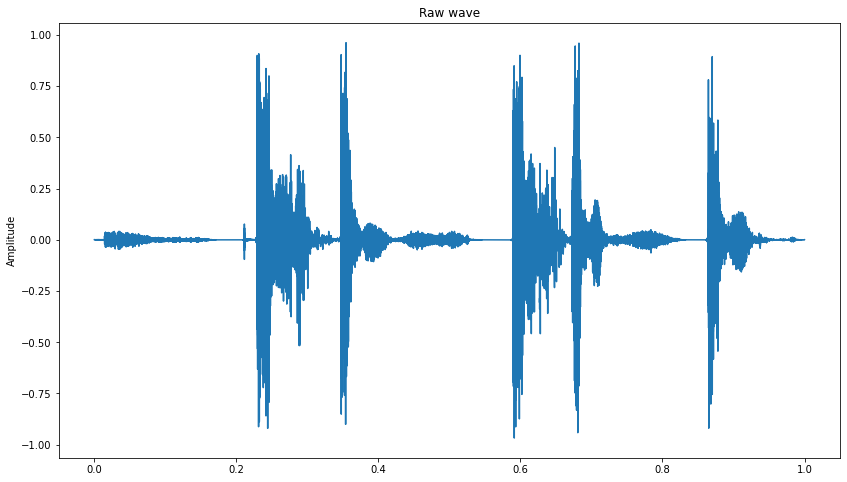
\includegraphics[width=11.8cm]{images/3.1.png}
\caption{Tín hiệu âm thanh gốc.}
\end{figure}
 
\begin{figure}[!h]
\captionsetup{width=0.8\textwidth}
\centering
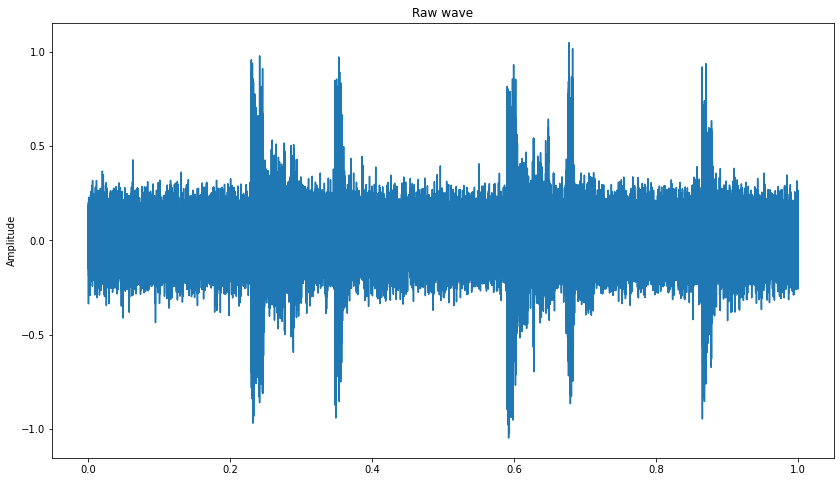
\includegraphics[width=12cm]{images/3.2.png}
\caption{Tín hiệu âm thanh sau khi thêm nhiễu.}
\end{figure}

\subsubsection{Dịch thời gian đoạn âm thanh}
Thực hiện dịch thời gian đoạn âm thanh với thời gian dịch tối đa là 80\% thời lượng của đoạn âm thanh. Chúng em tiến hành dịch âm thanh với thời gian ngẫu nhiên, dịch trái hay dịch phải cũng ngẫu nhiên với ngẫu nhiên khoảng 70\% tổng số dữ liêu gán nhãn dương tính trong tập huấn luyện.

\begin{figure}[!h]
\captionsetup{width=0.8\textwidth}
\centering
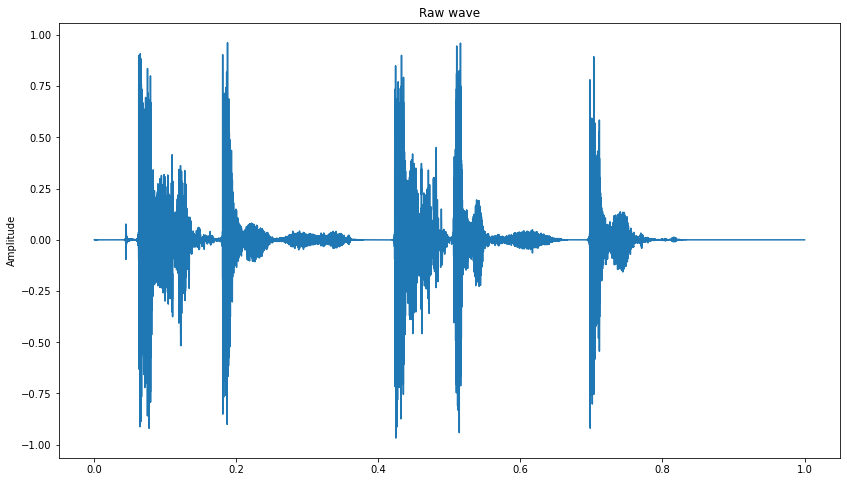
\includegraphics[width=12.5cm]{images/3.3.png}
\caption{Tín hiệu âm thanh sau khi dịch thời gian.}
\end{figure}


\subsubsection{Thay đổi cao độ đoạn âm thanh}
Thực hiện thay đổi cao độ đoạn âm thanh với hệ số thay đổi là 5. Cũng như hai phương pháp trên, nhóm thực hiện thay đổi độ cao với ngẫu nhiên khoảng 70\% tổng số dữ liêu gán nhãn dương tính trong tập huấn luyện.

\begin{figure}[!h]
\captionsetup{width=0.8\textwidth}
\centering
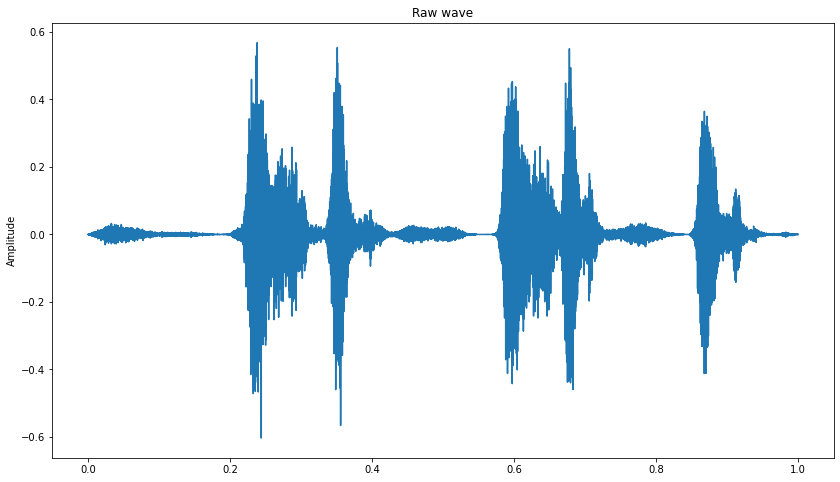
\includegraphics[width=12.5cm]{images/3.4.png}
\caption{Tín hiệu âm sau khi thay đổi cao độ.}
\end{figure}

Sau khi thực hiện làm giàu dữ liệu cho tập huấn luyện, số lượng nhãn dương tính bây giờ là 1,957 và số lượng nhãn âm tính giữ nguyên là 2,735. Tỉ lệ nhãn dương tính và nhãn âm tính lúc này là 4.2/5.8, đã đỡ mất cân bằng hơn so với trước khi làm giàu dữ liệu.

\section{Trích xuất đặc trưng}
\noindent
Đối với dữ liệu âm thanh, chúng ta cần thực hiện trích xuất đặc trưng của từng mẫu dữ liệu để đưa vào huấn luyện. Có rất nhiều phương pháp trích xuất đặc trưng khác nhau. Nhóm em đã thử nghiệm qua một số loại trích xuất đặc trưng khác nhau và lựa chọn ra ba loại trích xuất đặc trưng thường được sử dụng nhiều trong các bài toán với dữ liệu âm thanh.

\subsection{Đặc trưng quang phổ - spectrogram}
Quang phổ (spectrogram) biễn diễn độ lớn của tín hiệu theo thời gian ở các tần số khác nhau. Nếu như phổ chỉ cung cấp thông tin về giá trị năng lượng của tín hiệu ở các tần số khác nhau thì quang phổ trực quan hơn khi biểu diễn sự thay đổi năng lượng đó theo thời gian.

\begin{figure}[!h]
\captionsetup{width=0.8\textwidth}
\centering
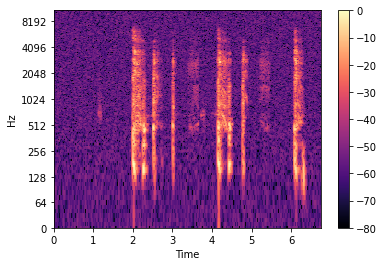
\includegraphics[width=12.5cm]{images/4.1.png}
\caption{Đặc trưng về quang phổ}
\end{figure}

\subsection{Đặc trưng Mel-frequency cepstral coefficients (MFCCs)}
Đặc trưng MFCCs sẽ chọn ra các hệ số (\textbf{coefficients} của phổ (\textbf{cepstral}) theo thang tần số Mel (\textbf{Mel-frequency}). Trước tiên, thực hiện biến đổi Fourier tín hiệu ngõ vào thu được phổ. Sau đó thực hiện lấy log các giá trị rồi ta thực hiện thay đổi thang tần số về thang tần số Mel.\\
Thang đo Mel được phát triển dựa trên thực tế về khả năng
phân biệt các tín hiệu tần số của con người \cite{stevens1937scale}. Ví dụ: con người có thể dễ dàng phân biệt sự khác nhau giữa hai tín hiệu có tần số 100Hz và 200Hz nhưng lại không thể phân biệt được sự khác nhau giữa hai tín hiệu có tần số 10000Hz và 10100Hz. Công thức chuyển đổi Hz sang Mel:
\begin{align*}
f_{Mel}  =1127 \log \left(1 + \frac{f_{Hz}}{700}  \right)
\end{align*}
\begin{figure}[!h]
\captionsetup{width=0.8\textwidth}
\centering
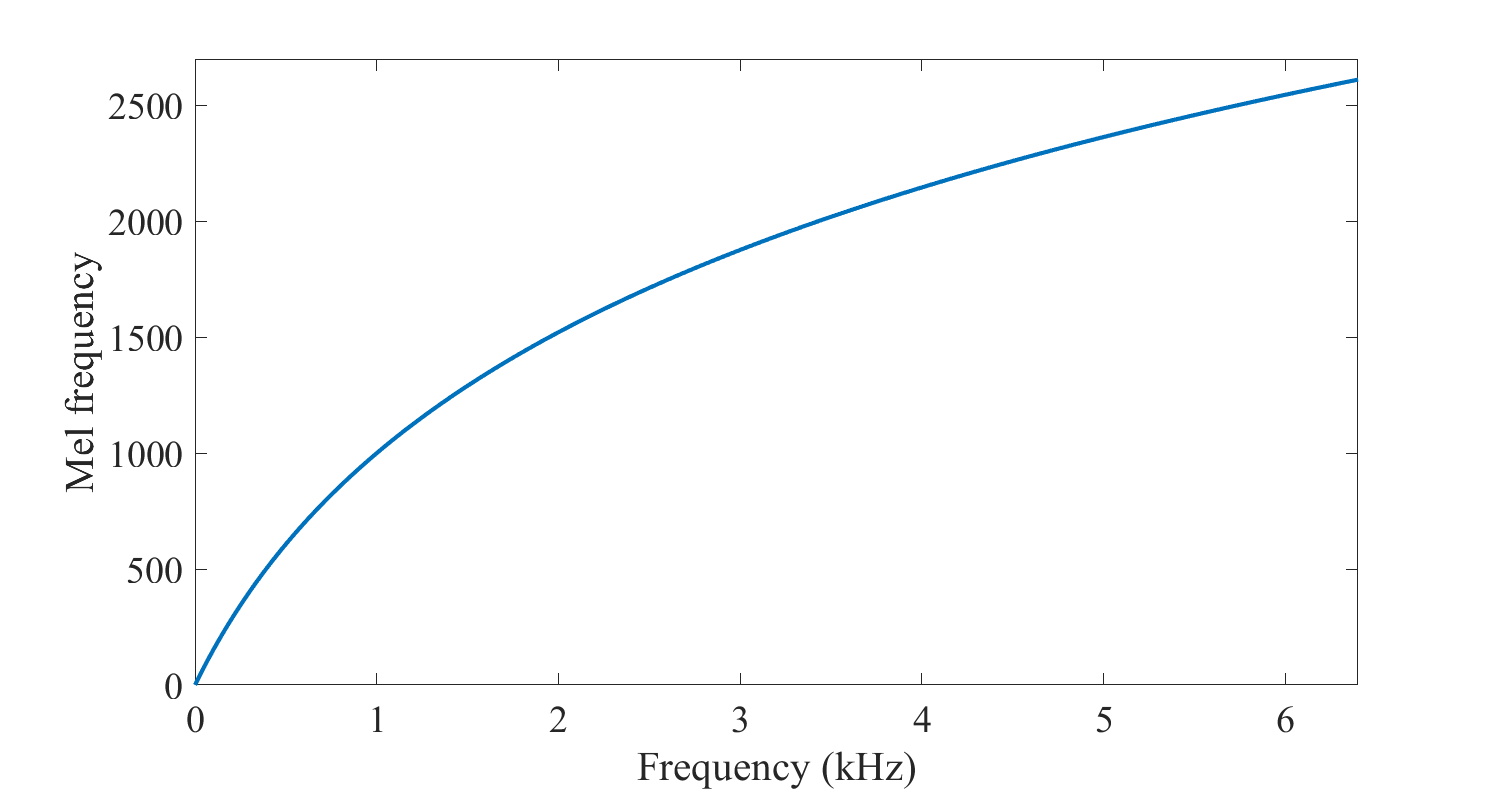
\includegraphics[width=11cm]{images/4.2.png}
\caption{Thang đo tần số Mel với thang đo Hz \cite{backstrom2019cepstrum}}
\end{figure}
Tín hiệu trong thực tế thường là tín hiệu không tuần huần hoàn, nên nếu ta áp dụng biến đổi Fourier cho toàn bộ tín hiệu có thể làm mất đi thông tin của tín hiệu. Do đó, ta thực hiện chia tín hiệu âm thanh đầu vào thành các khung nhỏ mỗi khung khoảng từ 20 đến 40ms để trích xuất đặc trưng. Sau khi chia các khung xong sẽ áp dụng cửa số Hamming lên để làm mượt các frame giúp tạo rõ tín hiệu, loại bỏ các thành phần nhiễu không cần thiết. Sau khi lấy Fourier tín hiệu rồi chuyển qua thang tần số Mel, tiếp theo ta sử dụng các filter bank dạng tam giác như hình 4.3 rồi cuối cùng sử dụng biến đổi cosine rời rạc (DCT) ta sẽ thu được kết quả MFCCs.

\begin{figure}[!h]
\captionsetup{width=0.8\textwidth}
\centering
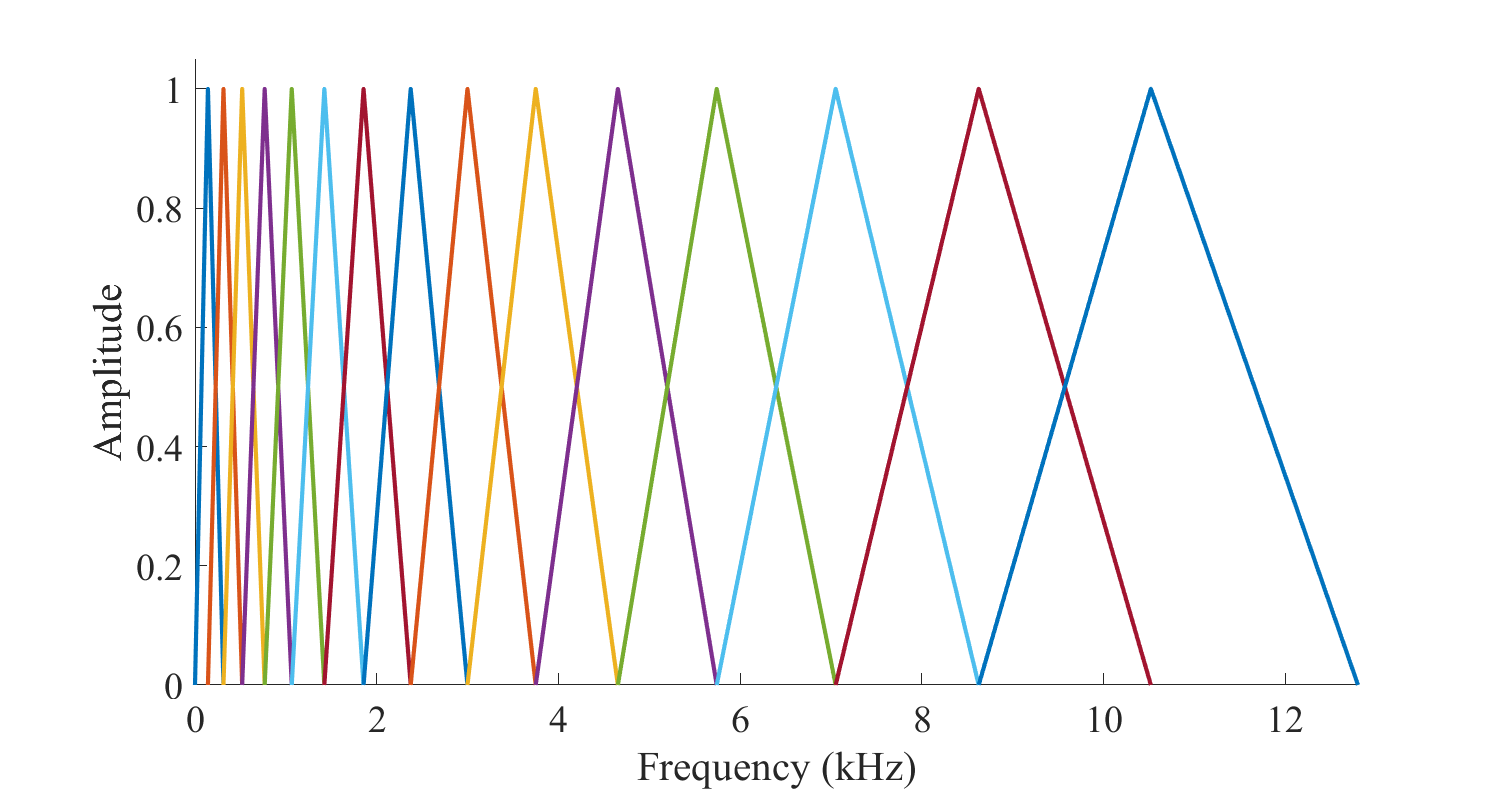
\includegraphics[width=10.5cm]{images/4.5.png}
\caption{Filter bank}
\end{figure}

\begin{figure}[!h]
\captionsetup{width=0.8\textwidth}
\centering
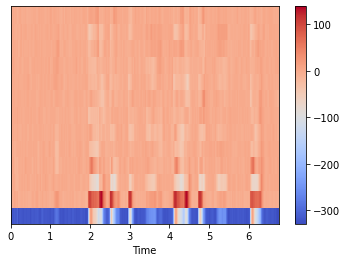
\includegraphics[width=12cm]{images/4.3.png}
\caption{Kết quả trích xuất MFCCs}
\end{figure}


\subsection{ Đặc trưng Sắc độ - Chroma}

Con người có thể cảm nhận được sự khác nhau cao độ của hai âm thanh khi chúng cách nhau một quảng tám (an octave), do đó cao độ của một âm có thể được tách ra làm hai phần là độ cao của âm (tone height) và sắc độ (chroma). Ta có 12 giá trị sắc độ được biểu diễn bởi tập hợp \{C, C\#, D, D\#, E , F, F\#, G, G\#, A, A\#, B \} phân bố trên dải tần số mà con người nghe được (từ 20Hz đến 20kHz). Ví dụ hình 4.5 nốt thứ nhất ta có C0 và C1 đều là nốt Đô (C) nhưng chúng cách nhau 12 nốt, nghĩa là tần số nốt C1 cao hơn so với tần số nốt C0. Tập hợp tất cả các giá trị cao độ của cùng một sắc độ được gọi là lớp cao độ (pitch class), ví dụ tập hợp $C: \{ C_n| n \in \mathbb{Z} \} = \{..., C_0, C_1, C_3, C_4, ... \}$ là tập hợp các cao độ của nốt Đô. 
\begin{figure}[!h]
\captionsetup{width=0.8\textwidth}
\centering
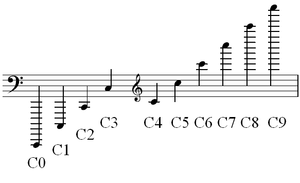
\includegraphics[width=10cm]{images/4.9.png}
\caption{Lớp cao độ của nốt Đô}
\end{figure}

\noindent
Đặc trưng sắc độ (chroma) sẽ phân tích phổ của tín hiệu âm thanh theo thang sắc độ thay vì thang tần số, ví dụ như hình 4.6.a là các nốt Đô, Rê, Mi, Pha, Son, La, Si, Đô. Hình 4.6.b là kết quả biễn diễn sắc độ lý tưởng cho hình 4.6.a. Khi biểu diễn cường độ tín hiệu theo thời gian trên phân tích phổ theo thang sắc độ được gọi là biểu đồ sắc độ của âm thanh. Ví dụ hình 4.7.c là một đoạn nhạc piano được biễn diễn trên miền thời gian, biểu đồ sắc độ của đoạn nhạc được thể hiện trên hình 4.6.d. 

\begin{figure}[!h]
\captionsetup{width=0.8\textwidth}
\centering
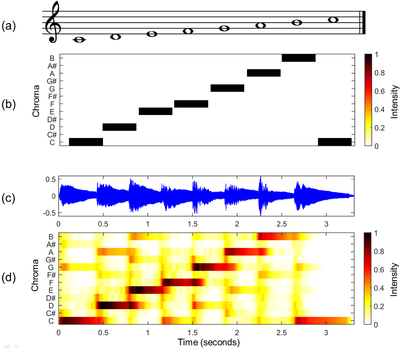
\includegraphics[width=12cm]{images/4.8.png}
\caption{Ví dụ về âm thanh phát ra của đàn piano}
\end{figure}

\begin{figure}[!h]
\captionsetup{width=0.8\textwidth}
\centering
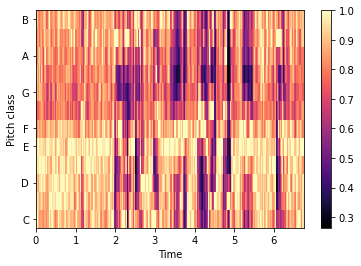
\includegraphics[width=12cm]{images/4.4.png}
\caption{Kết quả trích xuất đặc trưng Chroma}
\end{figure}

\section{Mô hình sử dụng}

\subsection{Mô hình thử nghiệm 1}

\noindent
Ở dạng mô hình thử nghiệm 1, chúng em sẽ sử dụng tách biệt từng đặc trưng để huấn luyện với mạng CNN dùng kỹ thuật học chuyển tiếp (transfer learning) dùng VGG16 với trọng số được huấn luyện từ tập Imagenet. Hình 5.1 là mô hình thử nghiệm với đặc trưng MFCC, sau khi ảnh đầu vào được đưa qua mạng VGG16 sẽ qua 1 tầng tích chập với 512 kernels có kernel\_size = 3, sau đó qua 1 lớp maxpooling với size = 2 và stride = 2. Tiếp theo, sử dụng kỹ thuật dropout với $p=0.3$ rồi dùng globalmaxpooling kết quả thu được một vector 512 phần tử. Sau đó, sẽ qua các lớp FCN (fully connected) với số node lần lượt là 128, 64, 16 với hàm kích hoạt là 'relu' và $dropout=0.5$. Cuối cùng đưa qua hàm softmax với 2 ngõ ra ứng với 2 lớp là dương tính (nhãn [0, 1]) và âm tính (nhãn [1, 0]).

\begin{figure}[!h]
\captionsetup{width=0.8\textwidth}
\centering
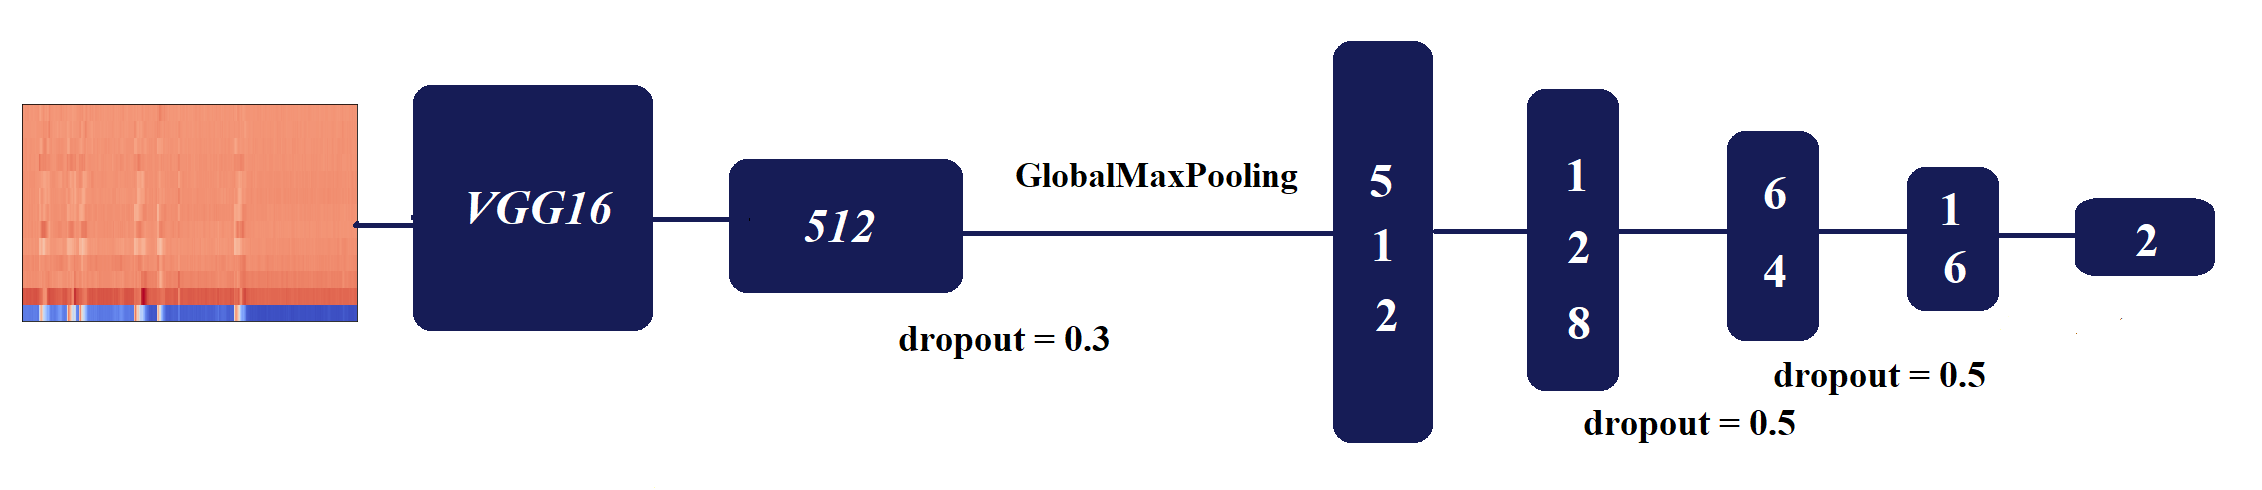
\includegraphics[width=15.5cm]{images/model 1.png}
\caption{Mô hình huấn luyện với đặc trưng MFCC}
\end{figure}

\noindent
Nhóm sử dụng hàm mất mát là cross-entropy, thuật toán tối ưu là Adam có hệ số học khởi tạo là 0.002, tiêu chí đánh giá là giá trị \textbf{auc}. Như đã trình bày ở trên, đối với tập dữ liệu y tế, mất cân bằng không thể dùng giá trị độ chính xác (accuracy) để đánh giá. Ngoài ra, chúng em sử dụng kỹ thuật smooth label để cải thiện hiệu quả của model \cite{DBLP:journals/corr/abs-1906-02629}.

\noindent
Thực hiện tương tự cho hai đặc trưng sắc độ (chroma) và quang phổ (spectogram) với cùng một mô hình nhưng chỉ thay đổi dạng đặc trưng ở ngõ vào.
\begin{figure}[!h]
\captionsetup{width=0.8\textwidth}
\centering
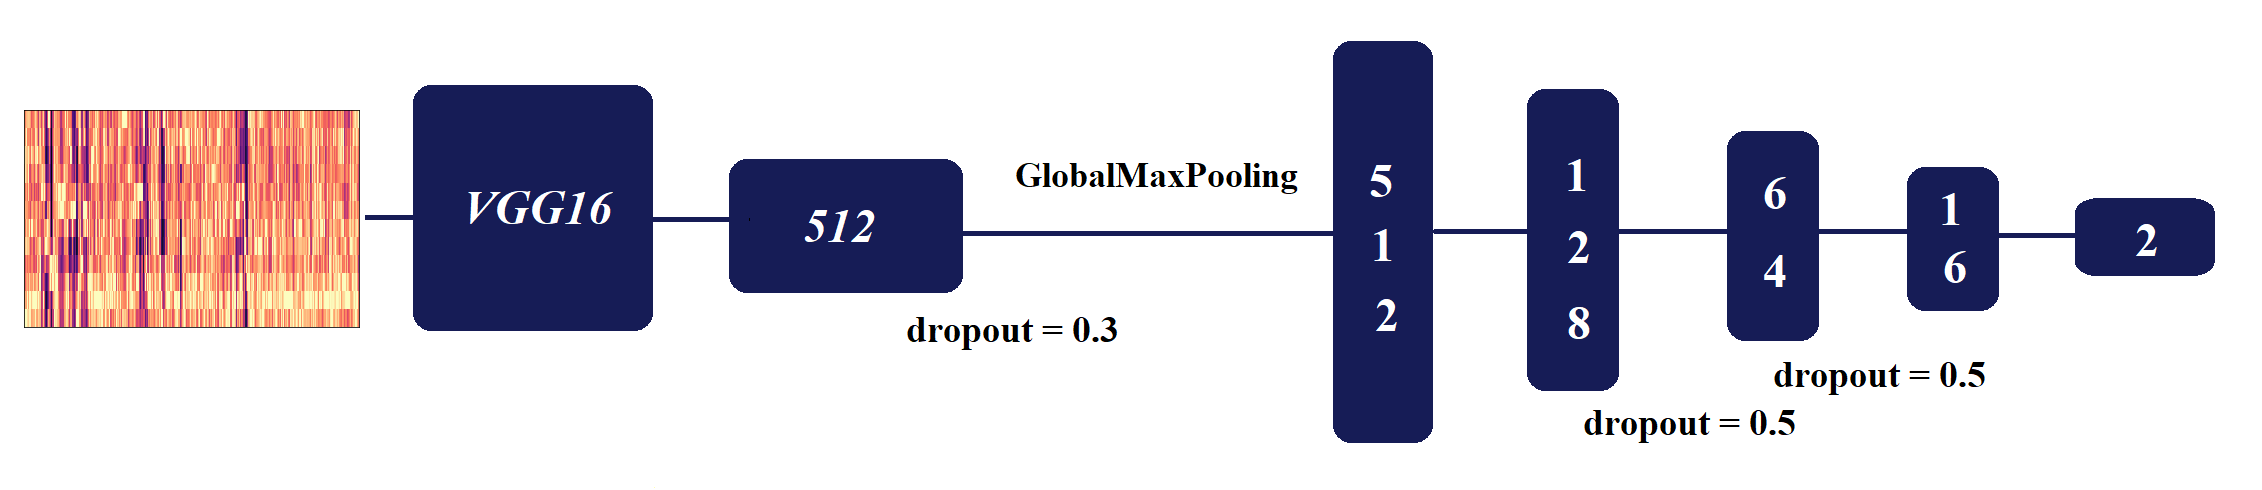
\includegraphics[width=15.5cm]{images/model 2.png}
\caption{Mô hình huấn luyện với đặc trưng Chroma.}
\end{figure}
\begin{figure}[!h]
\captionsetup{width=0.8\textwidth}
\centering
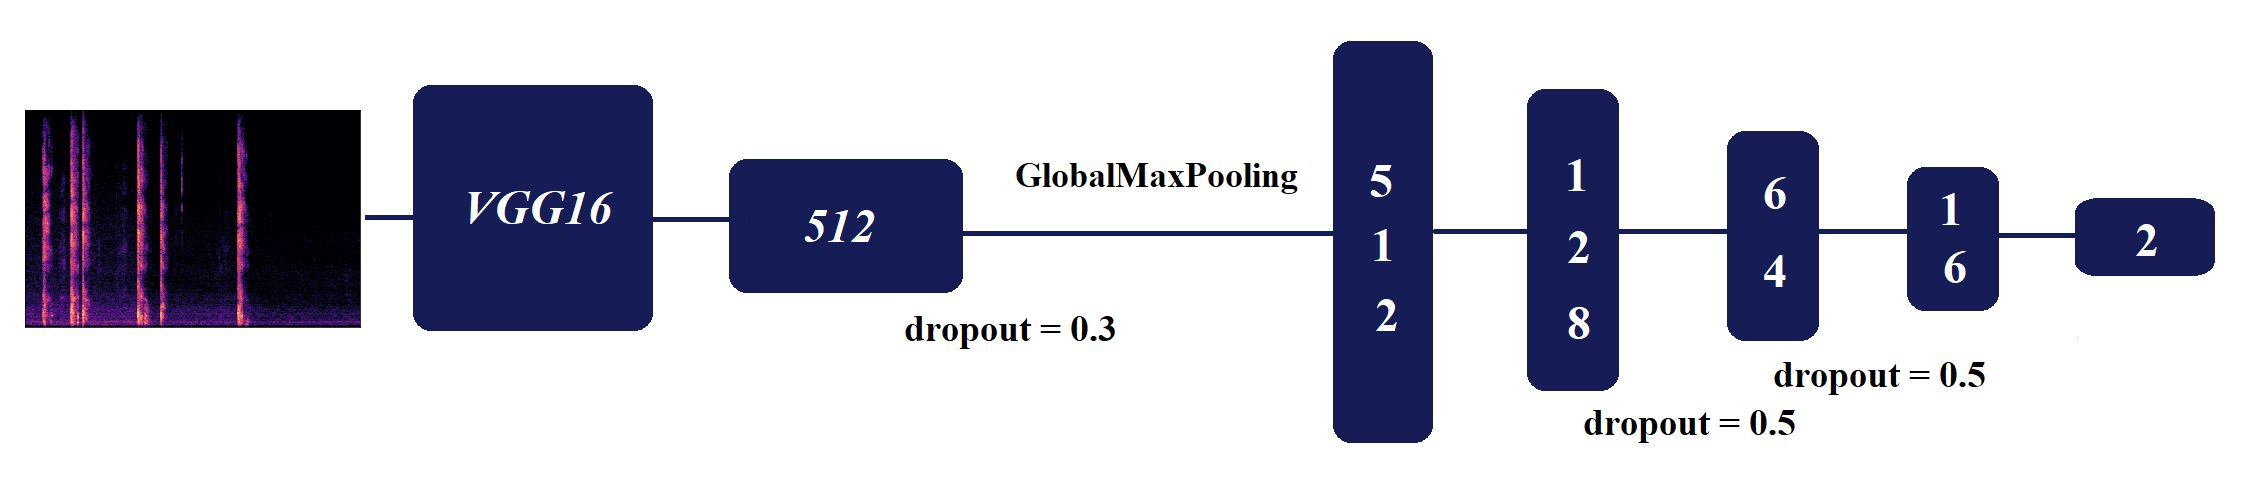
\includegraphics[width=15.5cm]{images/model 3.png}
\caption{Mô hình huấn luyện với đặc trưng Spectogram.}
\end{figure}


\subsection{Mô hình thử nghiệm 2}
Mô hình thử nghiệm 2 xuất phát từ ý tưởng kết hợp 3 đặc trưng với nhau. Sau khi đưa 3 đặc trưng (mỗi bộ 3 ảnh ở các đặc trưng ứng với một mẫu) qua một tầng tích chập được thiết kế giống nhau cho cả ba đặc trưng sau đó sẽ đi qua lớp globalmaxpooling với ngõ ra là một vector 256 phần tử. Sau đó tiến hành ghép (concate) ba vector này lại thành một vector có 768 phần tử, sau đó đi qua các lớp FCN với số node lần lượt là 128, 64, 16 với hàm kích hoạt là 'relu' và $dropout=0.5$. Cuối cùng đưa qua hàm softmax với 2 ngõ ra ứng với 2 lớp là dương tính (nhãn [0, 1]) và âm tính (nhãn [1, 0]).\\
\noindent
Về chi tiết mỗi trong khối CNN có 4 lớp CNN với số kernel lần lượt là 32, 64, 128, 256. Tất cả đều sử dụng kernel\_size = 3, hàm kích hoạt là 'leakyrelu' với hệ số $\alpha=0.2$, sau đó đi qua lớp maxpooling với size = 2 và stride = 2 và cuối cùng là dropout = 0.5. \\
\begin{figure}[!h]
\captionsetup{width=0.8\textwidth}
\centering
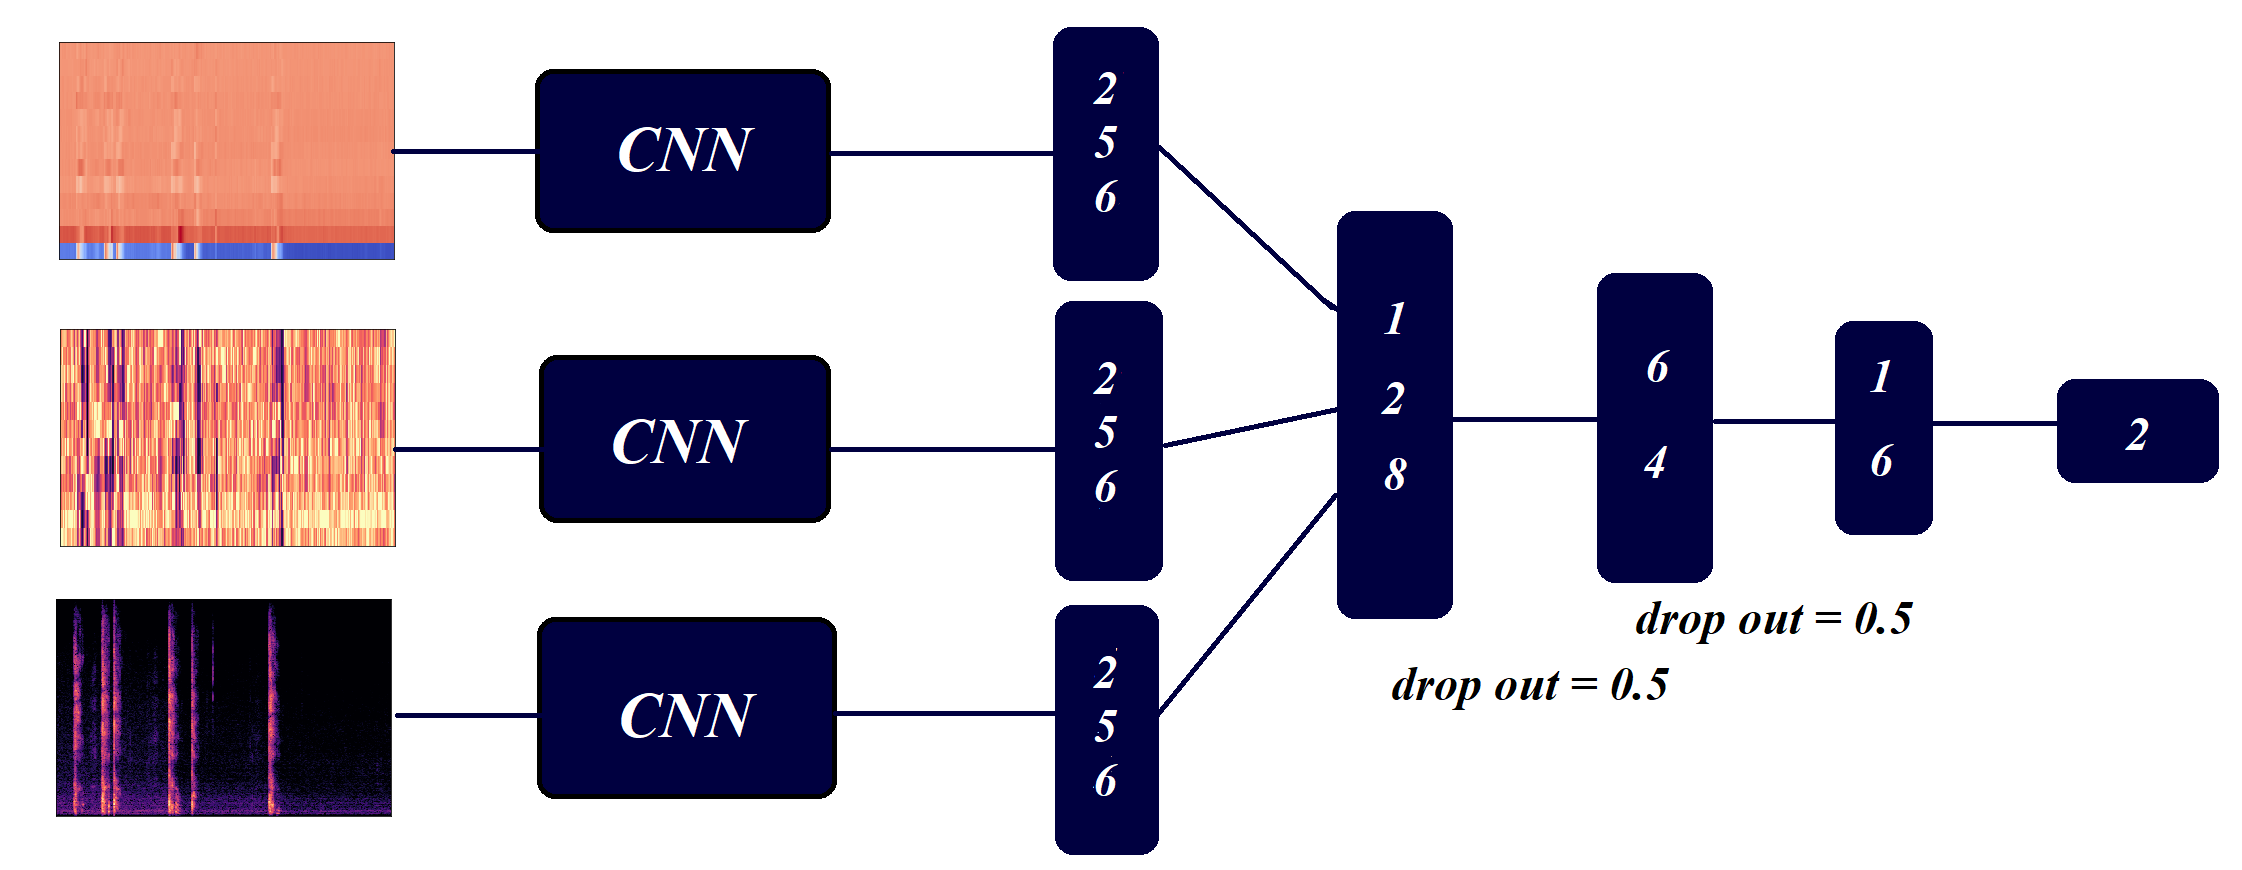
\includegraphics[width=17cm]{images/model 4.png}
\caption{Mô hình thử nghiệm kết hợp 3 đặc trưng.}
\end{figure}

\noindent
Khi triển khi mô hình này chúng em đã gặp một số khó khăn nhất định. Cụ thể như sau:

\begin{itemize}
    \item Thứ nhất, ban đầu khối CNN nhóm dự định sử dụng VGG-16 tuy nhiên do giới hạn của thư viện sử dụng nên 1 model chỉ được sử dụng 1 model học chuyển tiếp nên đã thay bằng một khối CNN đơn giản hơn để khảo sát.
    \item Thứ hai, do giới hạn về phần cứng nên cũng ảnh hưởng đến quá trình huấn luyện. Vì sử dụng kỹ thuật ghép (concate) nên không thể sử dụng các API high level để tải dữ liệu (có hỗ trợ tải dữ liệu tối ưu bộ nhớ) nên RAM của GPU dùng để huấn luyện (RAM do Google cung cấp trên Colab) bị tràn. Tổng số lượng ảnh nếu tải để huấn luyện khoảng 16k tấm, tuy nhiên khi tải được 5,000 tấm thì RAM bị tràn. Do đó, nhóm thực hiện chia nhỏ dữ liệu về huấn luyện tuần tự trên từng mẫu dữ liệu nhỏ. Nghĩa là sẽ huấn luyện trên bộ dự liệu nhỏ (khoảng 4,000 tấm cho cả ba đặc trưng) trong vài epoch rồi sau đó dùng kết quả đó tiếp tục huấn luyện với một tập dữ liệu nhỏ khác cho đến khi quét toàn bộ tập dữ liệu. Tiến hành thay đổi các cách kết hợp khác nhau và quét qua nhiều lần toàn bộ dữ liệu lớn để thu được kết quả cuối cùng.\\
\end{itemize}


\section{Kết quả và thảo luận}


\subsection{Kết quả thu được với mô hình thử nghiệm 1}

\subsubsection{Huấn luyện với đặc trưng MFCC}

\noindent
Kết quả sau khi huấn luyện đối với đặc trưng MFCC có confusion matrix và đường ROC thu được như hình 6.1.

\begin{figure}[!h]
\captionsetup{width=0.8\textwidth}
\centering
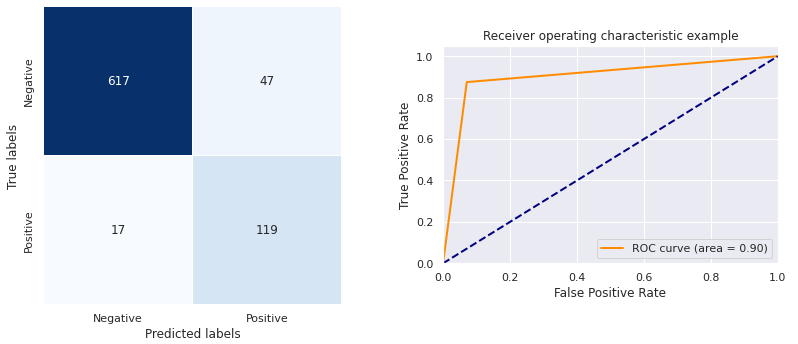
\includegraphics[width=17cm]{images/5.1.png}
\caption{Kết quả huấn luyện với đặc trưng MFCC.}
\end{figure}

Công thức tính một số thông số để đánh giá:
\begin{align*}
    Accuracy = \dfrac{617+119}{800} = 0.92\\
    Precision = \dfrac{119}{119+47} = 0.717\\
    Recall = \dfrac{119}{119+17} = 0.875\\
    F1-score = \dfrac{2\times0.717\times0.875}{0.717+0.875} = 0.788\\
    Specificity = \dfrac{617}{617+47}=0.929
\end{align*}

Từ confusion matrix cho thấy kết quả phân loại khá tốt khi xác định đúng 617 trường hợp âm tính thật và 119 trường hợp dương tính thật, xác định sai 47 trường hợp dương tính giả và 17 trường hợp âm tính giả. Thông số độ nhạy (recall) sau khi tính toán cũng cao, đạt 71.7\% và độ đặc hiệu (specificity) đạt 92.9\%. Tuy nhiên độ chính xác còn khá thấp chỉ 71.7\%.

\subsubsection{Huấn luyện với đặc trưng Chroma}
\noindent
Kết quả huấn luyện mô hình với đặc trưng sắc độ (chroma).

\begin{figure}[!h]
\captionsetup{width=0.8\textwidth}
\centering
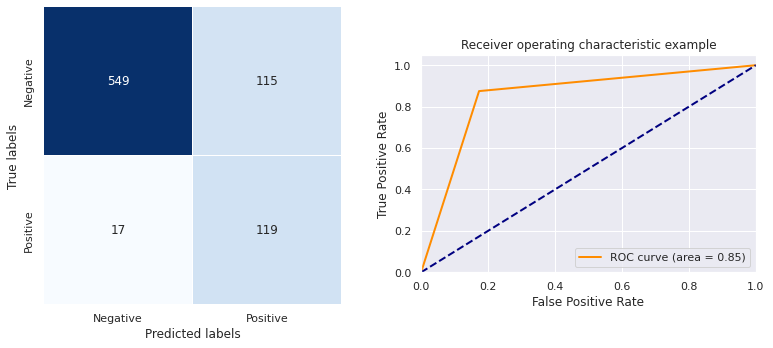
\includegraphics[width=17cm]{images/5.2.png}
\caption{Kết quả huấn luyện với đặc trưng Chroma}
\end{figure}

\begin{align*}
    Accuracy = \dfrac{549+119}{800} = 0.835\\
    Precision = \dfrac{119}{119+115} = 0.509\\
    Recall = \dfrac{119}{119+17} = 0.875\\
    F1-score = \dfrac{2\times0.509\times0.875}{0.509+0.875} = 0.643\\
    Specificity = \dfrac{549}{549+115}=0.827
\end{align*}

Mô hình đã phân loại đúng 549 trường hợp âm tính và 119 trường hợp dương tính, xác định sai 115 trường hợp dương tính giả và 17 trường hợp âm tính giả. Độ nhạy (recall) và độ đặc hiệu (specificity) cũng khá cao lần lượt đạt 87.5\% và 82.7\%. Tuy nhiên độ chính xác rất thấp chỉ có 50.9\%.


\subsubsection{Huấn luyện với đặc trưng Spectogram}
\noindent
Kết quả huấn luyện mô hình với đặc trưng quang phổ (spectogram).

\begin{figure}[!h]
\captionsetup{width=0.8\textwidth}
\centering
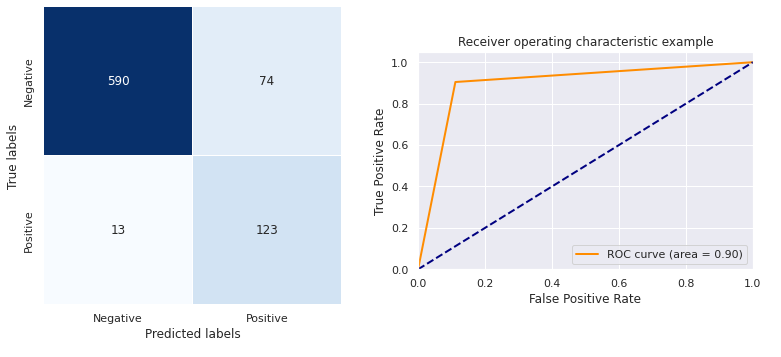
\includegraphics[width=16.5cm]{images/5.3.png}
\caption{Kết quả huấn luyện với đặc trưng Spectogram}
\end{figure}

\begin{align*}
    Accuracy = \dfrac{590+123}{800} = 0.891\\
    Precision = \dfrac{123}{123+74} = 0.624\\
    Recall = \dfrac{123}{123+13} = 0.904\\
    F1-score = \dfrac{2\times0.624\times0.904}{0.604+0.904} = 0.739\\
    Specificity = \dfrac{590}{590+74}=0.886
\end{align*}

Kết quả quan sát từ confusion matrix cho thấy mô hình đã phân loại đúng 590 trường hợp âm tính và 123 trường hợp dương tính, phân loại sai 74 trường hợp dương tính giả và 13 trường hợp âm tính giả. Kết quả tính toán độ nhạy rất tốt đạt 90.4\%, độ đặc hiệu cũng tương đối cao với 88.6\%. Tuy nhiên, độ chính xác còn khá thấp chỉ với 62.4\%.

\subsection{Kết quả thu được với mô hình thử nghiệm 2}

Tính toán một số thông số để đánh giá:

\begin{figure}[!h]
\captionsetup{width=0.8\textwidth}
\centering
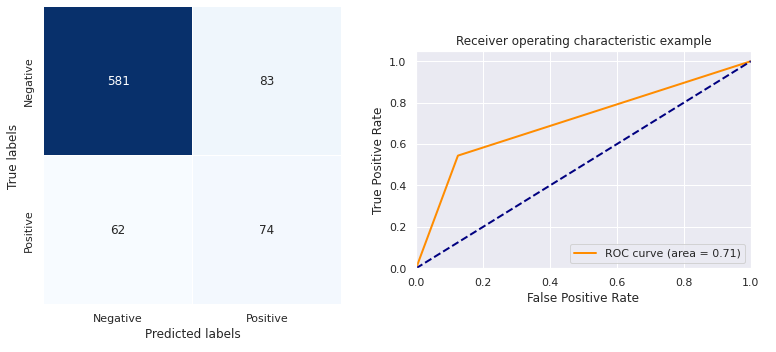
\includegraphics[width=16.5cm]{images/5.4.png}
\caption{Kết quả huấn luyện với mô hình thử nghiệm 2.}
\end{figure}

\begin{align*}
    Accuracy = \dfrac{581+74}{800} = 0.819\\
        Precision = \dfrac{74}{74+83} = 0.471
    \end{align*}
\begin{align*}
    Recall = \dfrac{74}{74+62} = 0.544\\
    F1-score = \dfrac{2\times0.471\times0.544}{0.471+0.544} = 0.505\\
    Specificity = \dfrac{581}{581+83}=0.875
\end{align*}

Mô hình phân loại đúng 581 trường hợp âm tính và 74 trường hợp dương tính, phân loại sai 83 trường hợp dương tính giả và 62 trường hợp âm tính giả. Kết quả độ nhạy (recall) và độ chính xác (precision) rất thấp, chỉ 54.4\% và 47.1\%.

\subsection{Nhận xét}

Sau khi huấn luyện mô hình với từng đặc trưng, chúng em đã tính toán các thông số đánh giá với kết quả dự đoán của tập kiểm thử. Tiếp theo, tiến hành kết hợp các vector softmax ngõ ra của 2 hoặc 3 đặc trưng (bằng cách cộng lại lấy trung bình) để đưa qua quyết định thay vì chỉ dùng kết quả của một đặc trưng duy nhất. Bảng kết quả đối với cả hai mô hình (Concatenate model là kết quả ứng với mô hình thử nghiệm 2).

\begin{table}[!h]
\centering
\begin{tabular}{|l|c|c|c|c|c|}
\hline
\multicolumn{1}{|c|}{\textit{\textbf{Model}}} & \multicolumn{1}{l|}{\textit{\textbf{Accuracy}}} & \multicolumn{1}{l|}{\textit{\textbf{Precision}}} & \multicolumn{1}{l|}{\textit{\textbf{Recall}}} & \multicolumn{1}{l|}{\textit{\textbf{F1-score}}} & \multicolumn{1}{l|}{\textit{\textbf{Specificity}}} \\ \hline
MFCC                                          & 0.92                                            & \textbf{0.717}                                   & 0.875                                         & 0.788                                           & 0.929                                              \\ \hline
Chroma                                        & 0.835                                           & 0.509                                            & 0.875                                         & 0.643                                           & 0.827                                              \\ \hline
Spectogram                                    & 0.891                                           & 0.624                                            & 0.904                                         & 0.739                                           & 0.886                                              \\ \hline
MFCC + Chroma                                 & 0.915                                           & 0.695                                            & 0.890                                         & 0.781                                           & 0.920                                              \\ \hline
MFCC + Spectogram                             & 0.934                                           & 0.758                                            & 0.897                                         & \textbf{0.822}                                  & \textbf{0.941}                                     \\ \hline
Chroma + Spectogram                           & 0.904                                           & 0.659                                            & 0.897                                         & 0.76                                            & 0.905                                              \\ \hline
MFCC + Chroma + Spec                    & 0.921                                           & 0.706                                            & \textbf{0.919}                                & 0.799                                           & 0.922                                              \\ \hline
Concatenate model                             & 0.819                                           & 0.471                                            & 0.544                                         & 0.505                                           & 0.875                                              \\ \hline
Giai đoạn 1                                   & \textbf{0.94}                                   & \textbf{0.82}                                    & \textbf{0.84}                                 & \textbf{0.83}                                   & \textbf{0.962}                                     \\ \hline
\end{tabular}
\caption{Bảng kết quả với hai mô hình thử nghiệm.}
\end{table}

\begin{figure}[!h]
\captionsetup{width=0.8\textwidth}
\centering
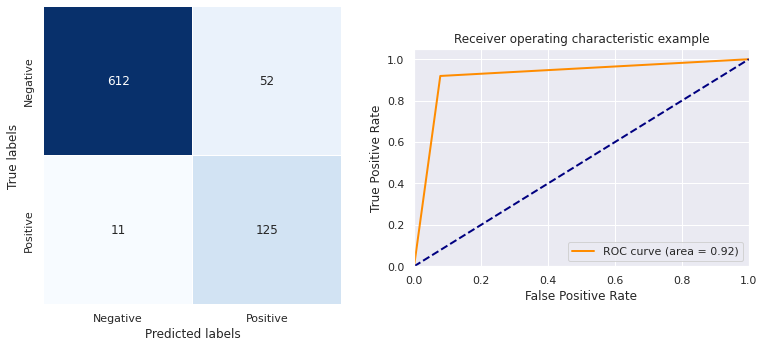
\includegraphics[width=16cm]{images/5.5.png}
\caption{Kết quả khi kết hợp ba đặc trưng ở mô hình 1.}
\end{figure}


\noindent
Trước tiên, đối với mô hình thử nghiệm 1 ở từng đặc trưng thì đặc trưng quang phổ (spectogram) có kết quả tốt hơn cả, độ nhạy (recall) đạt 90.4\%. Bởi như đã đề cập ở các phần trên, các phương pháp này xây dựng để có thể sàng lọc hết các trường hợp dương tính thật. Độ nhạy là tỉ lệ giữa số lượng dương tính thật trên tổng các số trường hợp dương tính, cho nên đối với các phương pháp sàng lọc giá trị này càng lớn càng tốt. Tuy nhiên, độ chính xác của của đặc trưng quang phổ không được tốt chỉ có 62.4\%, nghĩa là cứ trong 1000 người được xác định là dương tính thì chỉ có 624 người dương tính thật và có tới 376 người dương tính giả. Xét đến yếu tố độ chính xác này, thì đặc trưng MFCC cho kết quả tốt hơn với giá trị 71.7\% tuy nhiên giá trị độ nhạy lại thấp hơn 87.5\%. \\

\noindent
Với hy vọng đạt được kết quả tốt hơn, nhóm đã tiến hành cộng các vector softmax ở ngõ ra của 2 hoặc 3 đặc trưng để tiến hành đưa ra kết quả dự đoán. Cũng không ngoài dự đoán, kết quả khi xét hai đặc trưng MFCC và quang phổ cho kết quả F1-score tốt bởi một đặc trưng có độ chính xác cao và một đặc trưng có độ nhạy cao chúng ta hoàn toàn có thể hy vọng khi kết hợp sẽ được kết quả trung hòa với nhau. Kết quả độ nhạy đạt được 89.7\% cao hơn khi xét mỗi đặc trưng MFCC 2.2\%, và độ chính xác đạt 75.8\% cao hơn khi xét mỗi đặc trưng quang phổ tới 24.9\%. Độ đặc hiệu (specificity) của hai đặng trưng này khi kết hợp cũng rất cao lên đến 94.1\%. Tuy nhiên, kết quả khi kết hợp cả ba đặc trưng lại có độ nhạy rất cao 91.9\%, cao hơn 1.5\% so với xét mỗi đặc trưng quang phổ và cao hơn 2.2\% so với khi kết hợp hai đặc trưng quang phổ và MFCC. Nhưng độ chính xác và độ đặc hiệu khi xét đến sự kết hợp của ba đặc trưng lại thấp hơn so với sự kết hợp của hai đặc trưng quang phổ và MFCC.\\

\noindent
Mặc dù nhóm đã rất cố gắng trong quá trình huấn luyện mô hình thử nghiệm 2, tuy nhiên kết quả thu được không được tốt như mong muốn ban đầu. Kết quả thu được với độ nhạy khá thấp chỉ 54.4\%, nghĩa là nếu sử dụng kết quả này thì số lượng âm tính giả sẽ gần 50\% và kết quả sàng lọc sẽ rất tệ khi bỏ sót rất nhiều trường hợp dương tính. Bên cạnh đó, độ chính xác cũng rất thấp chỉ 47.1\% nghĩa là cứ 1000 người được xác định là dương tính thì chỉ có 471 người dương tính thật còn lại 529 người dương tính giả sẽ gây tốn kém chi phí xét nghiệm RT-PCR ở vòng tiếp theo. Do bị giới hạn về nhiều mặt nên nhóm em cũng không thể đưa kết luận chính xác nhất về việc mô hình kết hợp này có thật sự hoạt động hiệu quả hay không? Việc kết hợp 2 đặc trưng thay vì 3 đặc trưng sẽ cho kết quả như thế nào? \\

\noindent
So sánh với kết quả ở giai đoạn 1 (giai đoạn tham gia cuộc thi) thì kết quả cũng có phần cải thiện hơn. Độ nhạy của phương pháp mới này cao hơn so với giai đoạn trước 7.9\% (từ 84\% tăng lên 91.9\%) tuy nhiên độ chính xác lại giảm xuống 11.4\% (từ 82\% giảm xuống 70.6\%). Độ đặc hiệu của phương pháp mới cũng giảm 4\% từ 96.2\% xuống 92.2\%. Nhìn chung, hai phương pháp này đều có những ưu và nhược điểm điểm riêng. \\

\noindent
Với các kết quả đạt được, nhóm tin rằng việc áp dụng các mô hình trí tuện nhân tạo để phân loại sàng lọc người mắc bệnh COVID là khả thi. Nếu nghiên cứu và xây dựng một quy trình phù hợp, với chất lượng của đoạn âm thanh đầu vào tốt thì mô hình sẽ hoạt động hiệu quả. Việc này sẽ giảm bớt gánh nặng về tiền bạc trong vấn đề xét nghiệm nhanh hiện nay để tập trung vào việc tiêm chủng vacxin, đạt miễn dịch cộng đồng sớm nhất có thể.\\\

\newpage
\renewcommand{\bibname}{Tài liệu tham khảo}

%%%%%%%%%%%%%%%%%%%%%%%%%%%%%%%%%
\printbibliography

\end{document}